
%% corrfunc
\documentclass[twocolumn]{article}
\usepackage{graphicx}
\usepackage{xcolor}
\usepackage[margin=0.75in]{geometry}
\usepackage{float}
\usepackage{subcaption}
\usepackage{hyperref}
\newcommand\mynotes[1]{\textcolor{red}{#1}}
\author{Dan Korytov}
\title {\textbf{Core Compendium}:\\[.2em]Options on Fitting Cores to Data}

%%%%%%%%%%%%%%%%%%%%%%%
%% \pagecolor{black} %%
%% \color{white}     %%
%%%%%%%%%%%%%%%%%%%%%%%
\date{\today}


\begin{document}

\maketitle

\begin{abstract}
This document records the quality of fitting cores to red mapper
galaxy clusters. There are too many options and iterations to keep
everything in mind.
\end{abstract}


\section{Overview of options}
This section is broken down into two sections. The first section deals
with the creating the radial galaxy distribution the cores will try
to match. The second will go over the options on how to treat the
cores. 


\subsection{Target Galaxy Distribution Options}
These options are before we even use any core data. So combining all
these options with the options of how the cores are treated give us
the full option matrix.
\begin{itemize}
  
\item \textbf{Galaxy Luminosity}: The brightness relative to M* cut
  off for it to be counted in the stack. I've only looked at the two
  options below.  Most of the new core definition has been with Mr $<$
  M*.

  \begin{itemize}
    \item $\rm{M_{r} < M* }$
    \item $\rm{M_{r} < M*+1}$
  \end{itemize}
\item \textbf{Cluster Radial bins}: How the radial profile is
  stacked. Excluding the center did not change the fit significantly.
  \begin{itemize}
    \item 15 linear out to $\rm{R_{200}}$
    \item 15 linear from $0.05/0.1/0.2\rm{R_{200}}$ to $\rm{R_{200}}$
  \end{itemize}
\item \textbf{Cluster Mass Stacking}: How the clusters are stacked by
  SO mass. Currently, it's only done by log linear bins. It might be
  thinking about making the bins wider in the high mass region to
  reduce the uncertainty. Empty bins aren't taken into consideration
  for the fit.
  \begin{itemize}
    \item x log linear bins from 1e14 to 1e16 \mynotes{check}
  \end{itemize}
  
\item \textbf{Redshift Bins}: The clusters are stacked in redshift
  bins. There is almost no redshift evolution, so having only one
  redshift bin improves the statics.
  \begin{itemize}
    \item One bin from $0<z<0.35$
    \item Three bins from $0<0.10<0.20<0.3$
  \end{itemize}
\end{itemize}

%% \subsection{Core Catalog Generation Options}
%% Maybe it doesn't belong in this document--if this document is mainly about fitting cores
%% to data. 

%% \begin{itemize}

%% \item \textbf{Minimum Halo Mass for tracking}: Lower is better and
%%   more flexible, but requires more processing and storage. 
%%   \begin{itemize}
%%   \item 100 FoF Particles Halos 
%%   \end{itemize}

%% \item \textbf{Number of Core Partilces}: 
%%   \begin{itemize}
%%   \item 10
%%   \item 20
%%   \end{itemize}

%% \item \textbf{Definition of Radius}: Looked at the correlation of each radius
%%   definition as function of number of particles. 
%%   \begin{itemize}
%%   \item 50th, 60th, 80th percentile distance center
%%   \item RMS of the standard deviation in each dimension. -- currently use
%%   \item Average distance from the center
%%   \end{itemize}
  
%% \item \textbf{Central Core Treatment}: How are the central cores treated. The original
%%   method locked in the core particles after two+ halos merged with isolated central cores.
%%   So all the halo cores came from merger tree leaf nodes, which could be chronologically
%%   far away from the current halo time. A problem arose that some massive halos didn't have
%%   a compact core at the center. 
  
%%   \begin{itemize}
%%   \item No special treatment
%%   \item Force the backbone core to be at the halo center and be
%%     compact (implemented in the core fitting part)
%%   \item Centrals are refreshed at each time step -- currently used
%%   \end{itemize}
  
%% \end{itemize}

\subsection{Core Option}
\begin{itemize}
\item \textbf{Infall Mass Limit}: The minimum infall mass a core must posses
  for it be considered a candidate to be galaxy. Varying this infall
  mass while keeping other variables fixed, changes the overall
  abundance of cores in a cluster but does not change the shape of the
  profile significantly.
  \begin{itemize}
  \item On -- always required
  \end{itemize}

\item \textbf{Core Disruption Radius}: How diffuse can a candidate
  core be before it's considered disrupted and removed as a candidate
  for a galaxy.
  \begin{itemize}
  \item On
  \item Off -- current best fit
  \end{itemize}

\item \textbf{Core Merging Linking Length}: If two core candidates or
  more within are radius they are merged into one object. This uses an
  FoF merging algorithm for merging 3+ cores. The position is just the
  average position of the merged cores. \mynotes{Maybe weighted by
    infall mass so that centrals are weighted towards the center?}
  \begin{itemize}
  \item On -- current best fit
  \item Off 
  \end{itemize}
  

\item \textbf{Disrupted Cores Merging}: Allowing the particles of
  disrupted cores merge into a galaxy. There was a linking length and
  minimum number of particles required. This option was used to solve
  the missing central problem which was solved by refreshing central
  cores. 
  \begin{itemize}
  \item Off: not needed any more
  \end{itemize}

\item \textbf{Infall time pass?}: Maybe cores automatically
  disrupt/merge after a certain amount of time. Just a thought, not
  implemented.
  \begin{itemize}
  \item Off -- not implement 
  \end{itemize}

\item \textbf{Cluster Radius}: To construct the radial profile, all
  cores within a radius of the cluster center are used. I've tried
  some different radii and the parameters of the fit are pretty
  insensitive to the limit. Cores further out contribute a small fraction
  to the profile after smoothing for different angles. 
  \begin{itemize}
    \item 3 Mpc/h
    \item 5 Mpc/h
    \item 8 Mpc/h
  \end{itemize}
  
\end{itemize}


\subsection{Fit Option}
After deciding how the data and cores are treated, there are still
several options on how to calculate the likelihood function.

\begin{itemize}
  
\item \textbf{Fitting radial profile}: The main mode of fitting. Each
  stack of clusters try to match the radial surface density profiles
  of galaxies/cores.
  
\item \textbf{Fitting Ngal}: Fitting number of galaxies within
  R$_{200}$ per each stack of clusters to match. The disagreement is
  weighted equally as the radial bins. Each stack has ~15 radial bins
  errors and only 1 Ngal error, so it's a bit under
  weighted. \mynotes{Maybe this can work well with global abundance? Just as a
    side experiment}

  
\item \textbf{Fitting Accumulated Core profile}: Error bars are highly
  correlated and don't get the right treatment for the correlation. This is
  sort of an upweighted Ngal requirement. Just of exploratory fitting.
  

\item \textbf{Minimum Number of Clusters in Stack}: Some stacks of
  clusters have only a few clusters and might not representative of
  that stack. The Poisson error will be large, so they don't provide
  too strong of constraints. They could be excluded from the analysis
  complete or left in.
  \begin{itemize}
    \item No Requirement
    \item at least \mynotes{X}
  \end{itemize}


\item \textbf{Locking the Global Abundance}: Requires that the
  abundance of cores per unit volume to match the expected abundance
  of M*+x galaxies. This is done by fitting core disruption parameter
  while adjusting the infall mass to match the expected
  abundance. \textbf{Note}: While fitting for the abundance and
  profiles, we can't get a good fit to the profile. \mynotes{Is this
    only a two parameter fit? Can I look at merging as well?}


\item \textbf{Fitting Global Abundance}: Instead of locking the
  parameters to follow the global abundance of galaxies, the global
  abundance is taking into account for the likelihood evaluation. See
  \hyperref[sec:abundance example]{link\_to\_appendix}  for an example on the
  effect on the likelihood/ cost function. So far the fit looks pretty
  good. :)
%%TODO
%%Check that the link is working correctly. 

  
\item \textbf{2-point function}: Not implemented. 


\end{itemize}

%%%%%%%%%%%%%%%%%%%%%%%%%%%%%%%%%
%% Fit Procedure
%%%%%%%%%%%%%%%%%%%%%%%%%%%%%%%%%
\section{Fit Procedure}

\subsection{Error}
The RMS of the Poisson noise and error on the mean for each stacked radial bin.

\subsection{Posterior}
Either through MCMC or grid search. The low dimensionality of the
problem (only two or three parameters) lend to faster and more
accurate results by a flat grid search. 

\section{Fit Results}
\begin{figure}
  \includegraphics[width=0.6\textwidth]{figs/generate_parameter_dist.py/fig1.png}
  \caption{Model Parameters for fitting different data sets and
    models. The galaxies modeled in this figure are Mstar+0 galaxies. }
\end{figure}
\twocolumn
\clearpage
%%%%%%%%%%%%%%%%%%%%%%%%%%%%%%%%%
%% Appendix
%%%%%%%%%%%%%%%%%%%%%%%%%%%%%%%%%
\appendix


%%%%%%%%%%%%%%%%%%%%%%%%%%%%%%%%%
%% Red mapper basic distributions
%%%%%%%%%%%%%%%%%%%%%%%%%%%%%%%%%
%% \onecolumn
%% \section{RedMapper distributions}

%% \begin{figure}[H]
%%   \center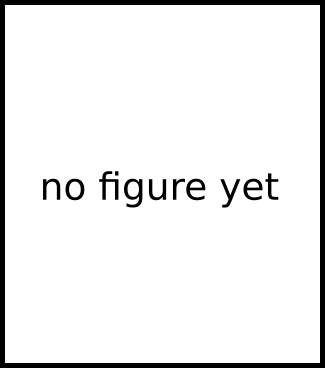
\includegraphics[width=0.4\textwidth]{figs/404.png}
%%   \caption{Redmapper cluster Redshift distribution}
%%   \label{fig:redmapper_redshift}
%% \end{figure}


%% \begin{figure}[H]
%%   \center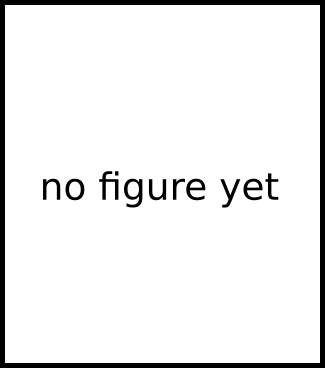
\includegraphics[width=0.4\textwidth]{figs/404.png}
%%   \caption{Redmapper cluster Mass distribution}
%%   \label{fig:redmapper_mass}
%% \end{figure}

%% \begin{figure}[H]
%%   \center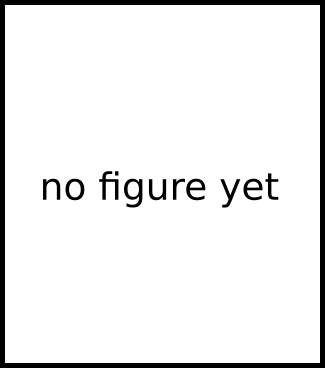
\includegraphics[width=0.4\textwidth]{figs/404.png}
%%   \caption{Redmapper cluster redshift and mass distribution}
%%   \label{fig:redmapper_redshift_mass}
%% \end{figure}

%% \begin{figure}[H]
%%   \center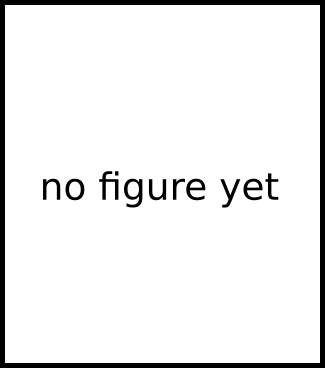
\includegraphics[width=0.4\textwidth]{figs/404.png}
%%   \caption{Calculated Richness vs Mass}
%%   \label{fig:redmapper_richness_mass}
%% \end{figure}

%% \clearpage

%%%%%%%%%%%%%%%%%%%%%%%%%%%%%%%%%
%% Simulation basic distributions
%%%%%%%%%%%%%%%%%%%%%%%%%%%%%%%%%
%% \section{Simulation Distributions}

%% \begin{figure}[H]
%%   \center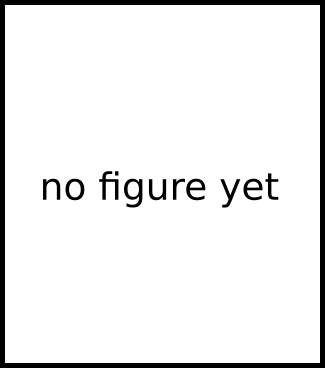
\includegraphics[width=0.4\textwidth]{figs/404.png}
%%   \caption{}
%%   \label{fig:simulation_mass_redshift}
%% \end{figure}

%% \clearpage


%%%%%%%%%%%%%%%%%%%%%%%%%%%%%%%%%
%% Basic Fit Disruption
%%%%%%%%%%%%%%%%%%%%%%%%%%%%%%%%%
\onecolumn
\section{Mstar+0, M200m}
\subsection{M200m, Mstar+0, Profile fit, Disruption Only}
\begin{figure}[H]
  \center\includegraphics[width=0.6\textwidth]{figs/params/cfn/simet/mstar0/mean/rd3.param/calc_likelihood_bounds.py/fig1.png}
  \caption{Likelihood on a parameter grid around the best mode. The marginalized parameter likelihood have
    1 $\sigma$ areas shaded in blue. The 2D likelihood distributions have 1 $\sigma$  and 2 $\sigma$ contours}
  \label{fig:basic_rd:likelihood}
\end{figure}

\begin{figure}[H]
  \center\includegraphics[width=0.6\textwidth]{figs/params/cfn/simet/mstar0/mean/rd3.param/calc_likelihood_bounds.py/fig2.png}
  \caption{Likelihood on a parameter grid around the best mode. The marginalized parameter likelihood have
    1 $\sigma$ areas shaded in blue. The 2D likelihood distributions have 1 $\sigma$  and 2 $\sigma$ contours}
  \label{fig:basic_rd:likelihood}
\end{figure}

\begin{figure}[H]
  \center\includegraphics[width=0.6\textwidth]{figs/params/cfn/simet/mstar0/mean/rd3_zoom.param/calc_likelihood_bounds.py/fig1.png}
  \caption{Likelihood on a parameter grid around the best mode. The marginalized parameter likelihood have
    1 $\sigma$ areas shaded in blue. The 2D likelihood distributions have 1 $\sigma$  and 2 $\sigma$ contours}
  \label{fig:basic_rd:likelihood}
\end{figure}

\begin{figure}[H]
  \center\includegraphics[width=0.6\textwidth]{figs/params/cfn/simet/mstar0/mean/rd3_zoom.param/calc_likelihood_bounds.py/fig2.png}
  \caption{Likelihood on a parameter grid around the best mode. The marginalized parameter likelihood have
    1 $\sigma$ areas shaded in blue. The 2D likelihood distributions have 1 $\sigma$  and 2 $\sigma$ contours}
  \label{fig:basic_rd:likelihood}
\end{figure}


\begin{figure}
  \begin{subfigure}{.5\textwidth}
    \centering\includegraphics[width=1.0\linewidth]{figs/params/cfn/simet/mstar0/mean/rd3.param/plot_zmrs.py/fig2.png}
    \caption{a}
  \end{subfigure}
  \begin{subfigure}{.5\textwidth}
    \centering\includegraphics[width=1.0\linewidth]{figs/params/cfn/simet/mstar0/mean/rd3.param/plot_zmrs.py/fig3.png}
    \caption{a}
  \end{subfigure}
  \begin{subfigure}{.5\textwidth}
    \centering\includegraphics[width=1.0\linewidth]{figs/params/cfn/simet/mstar0/mean/rd3.param/plot_zmrs.py/fig4.png}
    \caption{a}
  \end{subfigure}%
  \begin{subfigure}{.5\textwidth}
    \centering\includegraphics[width=1.0\linewidth]{figs/params/cfn/simet/mstar0/mean/rd3.param/plot_zmrs.py/fig5.png}
    \caption{a}
  \end{subfigure}
  \begin{subfigure}{.5\textwidth}
    \centering\includegraphics[width=1.0\linewidth]{figs/params/cfn/simet/mstar0/mean/rd3.param/plot_zmrs.py/fig6.png}
    \caption{a}
  \end{subfigure}
  
\end{figure}
\clearpage


\subsection{M200m, Mstar+0, Profile fit, Merging Only}
\begin{figure}[H]
  \center\includegraphics[width=0.6\textwidth]{figs/params/cfn/simet/mstar0/mean/rm3.param/calc_likelihood_bounds.py/fig1.png}
  \caption{Likelihood on a parameter grid around the best mode. The marginalized parameter likelihood have
    1 $\sigma$ areas shaded in blue. The 2D likelihood distributions have 1 $\sigma$  and 2 $\sigma$ contours}
  \label{fig:basic_rd:likelihood}
\end{figure}

\begin{figure}[H]
  \center\includegraphics[width=0.6\textwidth]{figs/params/cfn/simet/mstar0/mean/rm3.param/calc_likelihood_bounds.py/fig2.png}
  \caption{Likelihood on a parameter grid around the best mode. The marginalized parameter likelihood have
    1 $\sigma$ areas shaded in blue. The 2D likelihood distributions have 1 $\sigma$  and 2 $\sigma$ contours}
  \label{fig:basic_rd:likelihood}
\end{figure}

\begin{figure}[H]
  \center\includegraphics[width=0.6\textwidth]{figs/params/cfn/simet/mstar0/mean/rm3_zoom.param/calc_likelihood_bounds.py/fig1.png}
  \caption{Likelihood on a parameter grid around the best mode. The marginalized parameter likelihood have
    1 $\sigma$ areas shaded in blue. The 2D likelihood distributions have 1 $\sigma$  and 2 $\sigma$ contours}
  \label{fig:basic_rd:likelihood}
\end{figure}

\begin{figure}[H]
  \center\includegraphics[width=0.6\textwidth]{figs/params/cfn/simet/mstar0/mean/rm3_zoom.param/calc_likelihood_bounds.py/fig2.png}
  \caption{Likelihood on a parameter grid around the best mode. The marginalized parameter likelihood have
    1 $\sigma$ areas shaded in blue. The 2D likelihood distributions have 1 $\sigma$  and 2 $\sigma$ contours}
  \label{fig:basic_rd:likelihood}
\end{figure}


\begin{figure}
  \begin{subfigure}{.5\textwidth}
    \centering\includegraphics[width=1.0\linewidth]{figs/params/cfn/simet/mstar0/mean/rm3.param/plot_zmrs.py/fig2.png}
    \caption{a}
  \end{subfigure}
  \begin{subfigure}{.5\textwidth}
    \centering\includegraphics[width=1.0\linewidth]{figs/params/cfn/simet/mstar0/mean/rm3.param/plot_zmrs.py/fig3.png}
    \caption{a}
  \end{subfigure}
  \begin{subfigure}{.5\textwidth}
    \centering\includegraphics[width=1.0\linewidth]{figs/params/cfn/simet/mstar0/mean/rm3.param/plot_zmrs.py/fig4.png}
    \caption{a}
  \end{subfigure}%
  \begin{subfigure}{.5\textwidth}
    \centering\includegraphics[width=1.0\linewidth]{figs/params/cfn/simet/mstar0/mean/rm3.param/plot_zmrs.py/fig5.png}
    \caption{a}
  \end{subfigure}
  \begin{subfigure}{.5\textwidth}
    \centering\includegraphics[width=1.0\linewidth]{figs/params/cfn/simet/mstar0/mean/rm3.param/plot_zmrs.py/fig6.png}
    \caption{a}
  \end{subfigure}
  
\end{figure}
\clearpage


\subsection{M200m, Mstar+0, Profile fit, Disruption + Merging}
\begin{figure}[H]
  \center\includegraphics[width=0.6\textwidth]{figs/params/cfn/simet/mstar0/mean/rd_rm3.param/calc_likelihood_bounds.py/fig1.png}
  \caption{Likelihood on a parameter grid around the best mode. The marginalized parameter likelihood have
    1 $\sigma$ areas shaded in blue. The 2D likelihood distributions have 1 $\sigma$  and 2 $\sigma$ contours}
  \label{fig:basic_rd:likelihood}
\end{figure}

\begin{figure}[H]
  \center\includegraphics[width=0.6\textwidth]{figs/params/cfn/simet/mstar0/mean/rd_rm3.param/calc_likelihood_bounds.py/fig2.png}
  \caption{Likelihood on a parameter grid around the best mode. The marginalized parameter likelihood have
    1 $\sigma$ areas shaded in blue. The 2D likelihood distributions have 1 $\sigma$  and 2 $\sigma$ contours}
  \label{fig:basic_rd:likelihood}
\end{figure}

\begin{figure}[H]
  \center\includegraphics[width=0.6\textwidth]{figs/params/cfn/simet/mstar0/mean/rd_rm3_zoom.param/calc_likelihood_bounds.py/fig1.png}
  \caption{Likelihood on a parameter grid around the best mode. The marginalized parameter likelihood have
    1 $\sigma$ areas shaded in blue. The 2D likelihood distributions have 1 $\sigma$  and 2 $\sigma$ contours}
  \label{fig:basic_rd:likelihood}
\end{figure}

\begin{figure}[H]
  \center\includegraphics[width=0.6\textwidth]{figs/params/cfn/simet/mstar0/mean/rd_rm3_zoom.param/calc_likelihood_bounds.py/fig2.png}
  \caption{Likelihood on a parameter grid around the best mode. The marginalized parameter likelihood have
    1 $\sigma$ areas shaded in blue. The 2D likelihood distributions have 1 $\sigma$  and 2 $\sigma$ contours}
  \label{fig:basic_rd:likelihood}
\end{figure}


\begin{figure}
  \begin{subfigure}{.5\textwidth}
    \centering\includegraphics[width=1.0\linewidth]{figs/params/cfn/simet/mstar0/mean/rd_rm3.param/plot_zmrs.py/fig2.png}
    \caption{a}
  \end{subfigure}
  \begin{subfigure}{.5\textwidth}
    \centering\includegraphics[width=1.0\linewidth]{figs/params/cfn/simet/mstar0/mean/rd_rm3.param/plot_zmrs.py/fig3.png}
    \caption{a}
  \end{subfigure}
  \begin{subfigure}{.5\textwidth}
    \centering\includegraphics[width=1.0\linewidth]{figs/params/cfn/simet/mstar0/mean/rd_rm3.param/plot_zmrs.py/fig4.png}
    \caption{a}
  \end{subfigure}%
  \begin{subfigure}{.5\textwidth}
    \centering\includegraphics[width=1.0\linewidth]{figs/params/cfn/simet/mstar0/mean/rd_rm3.param/plot_zmrs.py/fig5.png}
    \caption{a}
  \end{subfigure}
  \begin{subfigure}{.5\textwidth}
    \centering\includegraphics[width=1.0\linewidth]{figs/params/cfn/simet/mstar0/mean/rd_rm3.param/plot_zmrs.py/fig6.png}
    \caption{a}
  \end{subfigure}
  
\end{figure}
\clearpage


%%%%%%%%%%%%%%%%%%%%%%%%%%%%%%%%%
%% Abundance
%%%%%%%%%%%%%%%%%%%%%%%%%%%%%%%%%


\subsection{M200m, Mstar+0, Profile + Abundance fit, Disruption Only}
\begin{figure}[H]
  \center\includegraphics[width=0.6\textwidth]{figs/params/cfn/simet/mstar0/mean/abund/rd3.param/calc_likelihood_bounds.py/fig1.png}
  \caption{Likelihood on a parameter grid around the best mode. The marginalized parameter likelihood have
    1 $\sigma$ areas shaded in blue. The 2D likelihood distributions have 1 $\sigma$  and 2 $\sigma$ contours}
  \label{fig:basic_rd:likelihood}
\end{figure}

\begin{figure}[H]
  \center\includegraphics[width=0.6\textwidth]{figs/params/cfn/simet/mstar0/mean/abund/rd3.param/calc_likelihood_bounds.py/fig2.png}
  \caption{Likelihood on a parameter grid around the best mode. The marginalized parameter likelihood have
    1 $\sigma$ areas shaded in blue. The 2D likelihood distributions have 1 $\sigma$  and 2 $\sigma$ contours}
  \label{fig:basic_rd:likelihood}
\end{figure}

\begin{figure}[H]
  \center\includegraphics[width=0.6\textwidth]{figs/params/cfn/simet/mstar0/mean/abund/rd3_zoom.param/calc_likelihood_bounds.py/fig1.png}
  \caption{Likelihood on a parameter grid around the best mode. The marginalized parameter likelihood have
    1 $\sigma$ areas shaded in blue. The 2D likelihood distributions have 1 $\sigma$  and 2 $\sigma$ contours}
  \label{fig:basic_rd:likelihood}
\end{figure}

\begin{figure}[H]
  \center\includegraphics[width=0.6\textwidth]{figs/params/cfn/simet/mstar0/mean/abund/rd3_zoom.param/calc_likelihood_bounds.py/fig2.png}
  \caption{Likelihood on a parameter grid around the best mode. The marginalized parameter likelihood have
    1 $\sigma$ areas shaded in blue. The 2D likelihood distributions have 1 $\sigma$  and 2 $\sigma$ contours}
  \label{fig:basic_rd:likelihood}
\end{figure}


\begin{figure}
  \begin{subfigure}{.5\textwidth}
    \centering\includegraphics[width=1.0\linewidth]{figs/params/cfn/simet/mstar0/mean/abund/rd3.param/plot_zmrs.py/fig2.png}
    \caption{a}
  \end{subfigure}
  \begin{subfigure}{.5\textwidth}
    \centering\includegraphics[width=1.0\linewidth]{figs/params/cfn/simet/mstar0/mean/abund/rd3.param/plot_zmrs.py/fig3.png}
    \caption{a}
  \end{subfigure}
  \begin{subfigure}{.5\textwidth}
    \centering\includegraphics[width=1.0\linewidth]{figs/params/cfn/simet/mstar0/mean/abund/rd3.param/plot_zmrs.py/fig4.png}
    \caption{a}
  \end{subfigure}%
  \begin{subfigure}{.5\textwidth}
    \centering\includegraphics[width=1.0\linewidth]{figs/params/cfn/simet/mstar0/mean/abund/rd3.param/plot_zmrs.py/fig5.png}
    \caption{a}
  \end{subfigure}
  \begin{subfigure}{.5\textwidth}
    \centering\includegraphics[width=1.0\linewidth]{figs/params/cfn/simet/mstar0/mean/abund/rd3.param/plot_zmrs.py/fig6.png}
    \caption{a}
  \end{subfigure}
\end{figure}
\clearpage


\subsection{M200m, Mstar+0, Profile + Abundancefit, Merging Only}
\begin{figure}[H]
  \center\includegraphics[width=0.6\textwidth]{figs/params/cfn/simet/mstar0/mean/abund/rm3.param/calc_likelihood_bounds.py/fig1.png}
  \caption{Likelihood on a parameter grid around the best mode. The marginalized parameter likelihood have
    1 $\sigma$ areas shaded in blue. The 2D likelihood distributions have 1 $\sigma$  and 2 $\sigma$ contours}
  \label{fig:basic_rd:likelihood}
\end{figure}

\begin{figure}[H]
  \center\includegraphics[width=0.6\textwidth]{figs/params/cfn/simet/mstar0/mean/abund/rm3.param/calc_likelihood_bounds.py/fig2.png}
  \caption{Likelihood on a parameter grid around the best mode. The marginalized parameter likelihood have
    1 $\sigma$ areas shaded in blue. The 2D likelihood distributions have 1 $\sigma$  and 2 $\sigma$ contours}
  \label{fig:basic_rd:likelihood}

\end{figure}

\begin{figure}[H]
  \center\includegraphics[width=0.6\textwidth]{figs/params/cfn/simet/mstar0/mean/abund/rm3_zoom.param/calc_likelihood_bounds.py/fig1.png}
  \caption{Likelihood on a parameter grid around the best mode. The marginalized parameter likelihood have
    1 $\sigma$ areas shaded in blue. The 2D likelihood distributions have 1 $\sigma$  and 2 $\sigma$ contours}
  \label{fig:basic_rd:likelihood}
\end{figure}

\begin{figure}[H]
  \center\includegraphics[width=0.6\textwidth]{figs/params/cfn/simet/mstar0/mean/abund/rm3_zoom.param/calc_likelihood_bounds.py/fig2.png}
  \caption{Likelihood on a parameter grid around the best mode. The marginalized parameter likelihood have
    1 $\sigma$ areas shaded in blue. The 2D likelihood distributions have 1 $\sigma$  and 2 $\sigma$ contours}
  \label{fig:basic_rd:likelihood}
\end{figure}

\begin{figure}
  \begin{subfigure}{.5\textwidth}
    \centering\includegraphics[width=1.0\linewidth]{figs/params/cfn/simet/mstar0/mean/abund/rm3.param/plot_zmrs.py/fig2.png}
    \caption{a}
  \end{subfigure}
  \begin{subfigure}{.5\textwidth}
    \centering\includegraphics[width=1.0\linewidth]{figs/params/cfn/simet/mstar0/mean/abund/rm3.param/plot_zmrs.py/fig3.png}
    \caption{a}
  \end{subfigure}
  \begin{subfigure}{.5\textwidth}
    \centering\includegraphics[width=1.0\linewidth]{figs/params/cfn/simet/mstar0/mean/abund/rm3.param/plot_zmrs.py/fig4.png}
    \caption{a}
  \end{subfigure}%
  \begin{subfigure}{.5\textwidth}
    \centering\includegraphics[width=1.0\linewidth]{figs/params/cfn/simet/mstar0/mean/abund/rm3.param/plot_zmrs.py/fig5.png}
    \caption{a}
  \end{subfigure}
  \begin{subfigure}{.5\textwidth}
    \centering\includegraphics[width=1.0\linewidth]{figs/params/cfn/simet/mstar0/mean/abund/rm3.param/plot_zmrs.py/fig6.png}
    \caption{a}
  \end{subfigure}
\end{figure}
\clearpage



\subsection{M200m, Mstar+0, Profile + Abundance fit, Disruption + Merging}
\begin{figure}[H]
  \center\includegraphics[width=0.6\textwidth]{figs/params/cfn/simet/mstar0/mean/abund/rd_rm3.param/calc_likelihood_bounds.py/fig1.png}
  \caption{Likelihood on a parameter grid around the best mode. The marginalized parameter likelihood have
    1 $\sigma$ areas shaded in blue. The 2D likelihood distributions have 1 $\sigma$  and 2 $\sigma$ contours}
  \label{fig:basic_rd:likelihood}
\end{figure}

\begin{figure}[H]
  \center\includegraphics[width=0.6\textwidth]{figs/params/cfn/simet/mstar0/mean/abund/rd_rm3.param/calc_likelihood_bounds.py/fig2.png}
  \caption{Likelihood on a parameter grid around the best mode. The marginalized parameter likelihood have
    1 $\sigma$ areas shaded in blue. The 2D likelihood distributions have 1 $\sigma$  and 2 $\sigma$ contours}
  \label{fig:basic_rd:likelihood}
\end{figure}

\begin{figure}[H]
  \center\includegraphics[width=0.6\textwidth]{figs/params/cfn/simet/mstar0/mean/abund/rd_rm3_zoom.param/calc_likelihood_bounds.py/fig1.png}
  \caption{Likelihood on a parameter grid around the best mode. The marginalized parameter likelihood have
    1 $\sigma$ areas shaded in blue. The 2D likelihood distributions have 1 $\sigma$  and 2 $\sigma$ contours}
  \label{fig:basic_rd:likelihood}
\end{figure}

\begin{figure}[H]
  \center\includegraphics[width=0.6\textwidth]{figs/params/cfn/simet/mstar0/mean/abund/rd_rm3_zoom.param/calc_likelihood_bounds.py/fig2.png}
  \caption{Likelihood on a parameter grid around the best mode. The marginalized parameter likelihood have
    1 $\sigma$ areas shaded in blue. The 2D likelihood distributions have 1 $\sigma$  and 2 $\sigma$ contours}
  \label{fig:basic_rd:likelihood}
\end{figure}

\begin{figure}
  \begin{subfigure}{.5\textwidth}
    \centering\includegraphics[width=1.0\linewidth]{figs/params/cfn/simet/mstar0/mean/abund/rd_rm3.param/plot_zmrs.py/fig2.png}
    \caption{a}
  \end{subfigure}
  \begin{subfigure}{.5\textwidth}
    \centering\includegraphics[width=1.0\linewidth]{figs/params/cfn/simet/mstar0/mean/abund/rd_rm3.param/plot_zmrs.py/fig3.png}
    \caption{a}
  \end{subfigure}
  \begin{subfigure}{.5\textwidth}
    \centering\includegraphics[width=1.0\linewidth]{figs/params/cfn/simet/mstar0/mean/abund/rd_rm3.param/plot_zmrs.py/fig4.png}
    \caption{a}
  \end{subfigure}%
  \begin{subfigure}{.5\textwidth}
    \centering\includegraphics[width=1.0\linewidth]{figs/params/cfn/simet/mstar0/mean/abund/rd_rm3.param/plot_zmrs.py/fig5.png}
    \caption{a}
  \end{subfigure}
  \begin{subfigure}{.5\textwidth}
    \centering\includegraphics[width=1.0\linewidth]{figs/params/cfn/simet/mstar0/mean/abund/rd_rm3.param/plot_zmrs.py/fig6.png}
    \caption{a}
  \end{subfigure}
\end{figure}
\clearpage


%%%%%%%%%%%%%%%%%%%%%%%%%%%%%%%%%
%% M200_crit
%%%%%%%%%%%%%%%%%%%%%%%%%%%%%%%%%

\section{M200c, Mstar+0}
\subsection{M200c, Mstar+0, Profile fit, Disruption Only}
\begin{figure}[H]
  \center\includegraphics[width=0.6\textwidth]{figs/params/cfn/simet/mstar0/crit/rd3.param/calc_likelihood_bounds.py/fig1.png}
  \caption{Likelihood on a parameter grid around the best mode. The marginalized parameter likelihood have
    1 $\sigma$ areas shaded in blue. The 2D likelihood distributions have 1 $\sigma$  and 2 $\sigma$ contours}
  \label{fig:basic_rd:likelihood}
\end{figure}

\begin{figure}[H]
  \center\includegraphics[width=0.6\textwidth]{figs/params/cfn/simet/mstar0/crit/rd3.param/calc_likelihood_bounds.py/fig2.png}
  \caption{Likelihood on a parameter grid around the best mode. The marginalized parameter likelihood have
    1 $\sigma$ areas shaded in blue. The 2D likelihood distributions have 1 $\sigma$  and 2 $\sigma$ contours}
  \label{fig:basic_rd:likelihood}
\end{figure}

\begin{figure}[H]
  \center\includegraphics[width=0.6\textwidth]{figs/params/cfn/simet/mstar0/crit/rd3_zoom.param/calc_likelihood_bounds.py/fig1.png}
  \caption{Likelihood on a parameter grid around the best mode. The marginalized parameter likelihood have
    1 $\sigma$ areas shaded in blue. The 2D likelihood distributions have 1 $\sigma$  and 2 $\sigma$ contours}
  \label{fig:basic_rd:likelihood}
\end{figure}

\begin{figure}[H]
  \center\includegraphics[width=0.6\textwidth]{figs/params/cfn/simet/mstar0/crit/rd3_zoom.param/calc_likelihood_bounds.py/fig2.png}
  \caption{Likelihood on a parameter grid around the best mode. The marginalized parameter likelihood have
    1 $\sigma$ areas shaded in blue. The 2D likelihood distributions have 1 $\sigma$  and 2 $\sigma$ contours}
  \label{fig:basic_rd:likelihood}
\end{figure}

\begin{figure}
  \begin{subfigure}{.5\textwidth}
    \centering\includegraphics[width=1.0\linewidth]{figs/params/cfn/simet/mstar0/crit/rd3.param/plot_zmrs.py/fig2.png}
    \caption{a}
  \end{subfigure}
  \begin{subfigure}{.5\textwidth}
    \centering\includegraphics[width=1.0\linewidth]{figs/params/cfn/simet/mstar0/crit/rd3.param/plot_zmrs.py/fig3.png}
    \caption{a}
  \end{subfigure}
  \begin{subfigure}{.5\textwidth}
    \centering\includegraphics[width=1.0\linewidth]{figs/params/cfn/simet/mstar0/crit/rd3.param/plot_zmrs.py/fig4.png}
    \caption{a}
  \end{subfigure}%
  \begin{subfigure}{.5\textwidth}
    \centering\includegraphics[width=1.0\linewidth]{figs/params/cfn/simet/mstar0/crit/rd3.param/plot_zmrs.py/fig5.png}
    \caption{a}
  \end{subfigure}
  \begin{subfigure}{.5\textwidth}
    \centering\includegraphics[width=1.0\linewidth]{figs/params/cfn/simet/mstar0/crit/rd3.param/plot_zmrs.py/fig6.png}
    \caption{a}
  \end{subfigure}
\end{figure}
\clearpage



\subsection{M200c, Mstar+0, Profile fit, Merging Only}
\begin{figure}[H]
  \center\includegraphics[width=0.6\textwidth]{figs/params/cfn/simet/mstar0/crit/rm3.param/calc_likelihood_bounds.py/fig1.png}
  \caption{Likelihood on a parameter grid around the best mode. The marginalized parameter likelihood have
    1 $\sigma$ areas shaded in blue. The 2D likelihood distributions have 1 $\sigma$  and 2 $\sigma$ contours}
  \label{fig:basic_rd:likelihood}
\end{figure}

\begin{figure}[H]
  \center\includegraphics[width=0.6\textwidth]{figs/params/cfn/simet/mstar0/crit/rm3.param/calc_likelihood_bounds.py/fig2.png}
  \caption{Likelihood on a parameter grid around the best mode. The marginalized parameter likelihood have
    1 $\sigma$ areas shaded in blue. The 2D likelihood distributions have 1 $\sigma$  and 2 $\sigma$ contours}
  \label{fig:basic_rd:likelihood}
\end{figure}

\begin{figure}[H]
  \center\includegraphics[width=0.6\textwidth]{figs/params/cfn/simet/mstar0/crit/rm3_zoom.param/calc_likelihood_bounds.py/fig1.png}
  \caption{Likelihood on a parameter grid around the best mode. The marginalized parameter likelihood have
    1 $\sigma$ areas shaded in blue. The 2D likelihood distributions have 1 $\sigma$  and 2 $\sigma$ contours}
  \label{fig:basic_rd:likelihood}
\end{figure}

\begin{figure}[H]
  \center\includegraphics[width=0.6\textwidth]{figs/params/cfn/simet/mstar0/crit/rm3_zoom.param/calc_likelihood_bounds.py/fig2.png}
  \caption{Likelihood on a parameter grid around the best mode. The marginalized parameter likelihood have
    1 $\sigma$ areas shaded in blue. The 2D likelihood distributions have 1 $\sigma$  and 2 $\sigma$ contours}
  \label{fig:basic_rd:likelihood}
\end{figure}

\begin{figure}
  \begin{subfigure}{.5\textwidth}
    \centering\includegraphics[width=1.0\linewidth]{figs/params/cfn/simet/mstar0/crit/rm3.param/plot_zmrs.py/fig2.png}
    \caption{a}
  \end{subfigure}
  \begin{subfigure}{.5\textwidth}
    \centering\includegraphics[width=1.0\linewidth]{figs/params/cfn/simet/mstar0/crit/rm3.param/plot_zmrs.py/fig3.png}
    \caption{a}
  \end{subfigure}
  \begin{subfigure}{.5\textwidth}
    \centering\includegraphics[width=1.0\linewidth]{figs/params/cfn/simet/mstar0/crit/rm3.param/plot_zmrs.py/fig4.png}
    \caption{a}
  \end{subfigure}%
  \begin{subfigure}{.5\textwidth}
    \centering\includegraphics[width=1.0\linewidth]{figs/params/cfn/simet/mstar0/crit/rm3.param/plot_zmrs.py/fig5.png}
    \caption{a}
  \end{subfigure}
  \begin{subfigure}{.5\textwidth}
    \centering\includegraphics[width=1.0\linewidth]{figs/params/cfn/simet/mstar0/crit/rm3.param/plot_zmrs.py/fig6.png}
    \caption{a}
  \end{subfigure}
\end{figure}
\clearpage


\subsection{M200c, Mstar+0, Profile fit, Disruption + Merging}
\begin{figure}[H]
  \center\includegraphics[width=0.6\textwidth]{figs/params/cfn/simet/mstar0/crit/rd_rm3.param/calc_likelihood_bounds.py/fig1.png}
  \caption{Likelihood on a parameter grid around the best mode. The marginalized parameter likelihood have
    1 $\sigma$ areas shaded in blue. The 2D likelihood distributions have 1 $\sigma$  and 2 $\sigma$ contours}
  \label{fig:basic_rd:likelihood}
\end{figure}

\begin{figure}[H]
  \center\includegraphics[width=0.6\textwidth]{figs/params/cfn/simet/mstar0/crit/rd_rm3.param/calc_likelihood_bounds.py/fig2.png}
  \caption{Likelihood on a parameter grid around the best mode. The marginalized parameter likelihood have
    1 $\sigma$ areas shaded in blue. The 2D likelihood distributions have 1 $\sigma$  and 2 $\sigma$ contours}
  \label{fig:basic_rd:likelihood}
\end{figure}

\begin{figure}[H]
  \center\includegraphics[width=0.6\textwidth]{figs/params/cfn/simet/mstar0/crit/rd_rm3_zoom.param/calc_likelihood_bounds.py/fig1.png}
  \caption{Likelihood on a parameter grid around the best mode. The marginalized parameter likelihood have
    1 $\sigma$ areas shaded in blue. The 2D likelihood distributions have 1 $\sigma$  and 2 $\sigma$ contours}
  \label{fig:basic_rd:likelihood}
\end{figure}

\begin{figure}[H]
  \center\includegraphics[width=0.6\textwidth]{figs/params/cfn/simet/mstar0/crit/rd_rm3_zoom.param/calc_likelihood_bounds.py/fig2.png}
  \caption{Likelihood on a parameter grid around the best mode. The marginalized parameter likelihood have
    1 $\sigma$ areas shaded in blue. The 2D likelihood distributions have 1 $\sigma$  and 2 $\sigma$ contours}
  \label{fig:basic_rd:likelihood}
\end{figure}

\begin{figure}
  \begin{subfigure}{.5\textwidth}
    \centering\includegraphics[width=1.0\linewidth]{figs/params/cfn/simet/mstar0/crit/rd_rm3.param/plot_zmrs.py/fig2.png}
    \caption{a}
  \end{subfigure}
  \begin{subfigure}{.5\textwidth}
    \centering\includegraphics[width=1.0\linewidth]{figs/params/cfn/simet/mstar0/crit/rd_rm3.param/plot_zmrs.py/fig3.png}
    \caption{a}
  \end{subfigure}
  \begin{subfigure}{.5\textwidth}
    \centering\includegraphics[width=1.0\linewidth]{figs/params/cfn/simet/mstar0/crit/rd_rm3.param/plot_zmrs.py/fig4.png}
    \caption{a}
  \end{subfigure}%
  \begin{subfigure}{.5\textwidth}
    \centering\includegraphics[width=1.0\linewidth]{figs/params/cfn/simet/mstar0/crit/rd_rm3.param/plot_zmrs.py/fig5.png}
    \caption{a}
  \end{subfigure}
  \begin{subfigure}{.5\textwidth}
    \centering\includegraphics[width=1.0\linewidth]{figs/params/cfn/simet/mstar0/crit/rd_rm3.param/plot_zmrs.py/fig6.png}
    \caption{a}
  \end{subfigure}
\end{figure}
\clearpage

\subsection{M200c, Mstar+0, Profile + Abundance, Disruption Only}
\begin{figure}[H]
  \center\includegraphics[width=0.6\textwidth]{figs/params/cfn/simet/mstar0/crit/abund/rd3.param/calc_likelihood_bounds.py/fig1.png}
  \caption{Likelihood on a parameter grid around the best mode. The marginalized parameter likelihood have
    1 $\sigma$ areas shaded in blue. The 2D likelihood distributions have 1 $\sigma$  and 2 $\sigma$ contours}
  \label{fig:basic_rd:likelihood}
\end{figure}

\begin{figure}[H]
  \center\includegraphics[width=0.6\textwidth]{figs/params/cfn/simet/mstar0/crit/abund/rd3.param/calc_likelihood_bounds.py/fig2.png}
  \caption{Likelihood on a parameter grid around the best mode. The marginalized parameter likelihood have
    1 $\sigma$ areas shaded in blue. The 2D likelihood distributions have 1 $\sigma$  and 2 $\sigma$ contours}
  \label{fig:basic_rd:likelihood}
\end{figure}

\begin{figure}[H]
  \center\includegraphics[width=0.6\textwidth]{figs/params/cfn/simet/mstar0/crit/abund/rd3_zoom.param/calc_likelihood_bounds.py/fig1.png}
  \caption{Likelihood on a parameter grid around the best mode. The marginalized parameter likelihood have
    1 $\sigma$ areas shaded in blue. The 2D likelihood distributions have 1 $\sigma$  and 2 $\sigma$ contours}
  \label{fig:basic_rd:likelihood}
\end{figure}

\begin{figure}[H]
  \center\includegraphics[width=0.6\textwidth]{figs/params/cfn/simet/mstar0/crit/abund/rd3_zoom.param/calc_likelihood_bounds.py/fig2.png}
  \caption{Likelihood on a parameter grid around the best mode. The marginalized parameter likelihood have
    1 $\sigma$ areas shaded in blue. The 2D likelihood distributions have 1 $\sigma$  and 2 $\sigma$ contours}
  \label{fig:basic_rd:likelihood}
\end{figure}

\begin{figure}
  \begin{subfigure}{.5\textwidth}
    \centering\includegraphics[width=1.0\linewidth]{figs/params/cfn/simet/mstar0/crit/abund/rd3.param/plot_zmrs.py/fig2.png}
    \caption{a}
  \end{subfigure}
  \begin{subfigure}{.5\textwidth}
    \centering\includegraphics[width=1.0\linewidth]{figs/params/cfn/simet/mstar0/crit/abund/rd3.param/plot_zmrs.py/fig3.png}
    \caption{a}
  \end{subfigure}
  \begin{subfigure}{.5\textwidth}
    \centering\includegraphics[width=1.0\linewidth]{figs/params/cfn/simet/mstar0/crit/abund/rd3.param/plot_zmrs.py/fig4.png}
    \caption{a}
  \end{subfigure}%
  \begin{subfigure}{.5\textwidth}
    \centering\includegraphics[width=1.0\linewidth]{figs/params/cfn/simet/mstar0/crit/abund/rd3.param/plot_zmrs.py/fig5.png}
    \caption{a}
  \end{subfigure}
  \begin{subfigure}{.5\textwidth}
    \centering\includegraphics[width=1.0\linewidth]{figs/params/cfn/simet/mstar0/crit/abund/rd3.param/plot_zmrs.py/fig6.png}
    \caption{a}
  \end{subfigure}
\end{figure}
\clearpage



\subsection{M200c, Mstar+0, Profile + Abundance, Merging Only}
\begin{figure}[H]
  \center\includegraphics[width=0.6\textwidth]{figs/params/cfn/simet/mstar0/crit/abund/rm3.param/calc_likelihood_bounds.py/fig1.png}
  \caption{Likelihood on a parameter grid around the best mode. The marginalized parameter likelihood have
    1 $\sigma$ areas shaded in blue. The 2D likelihood distributions have 1 $\sigma$  and 2 $\sigma$ contours}
  \label{fig:basic_rd:likelihood}
\end{figure}

\begin{figure}[H]
  \center\includegraphics[width=0.6\textwidth]{figs/params/cfn/simet/mstar0/crit/abund/rm3.param/calc_likelihood_bounds.py/fig2.png}
  \caption{Likelihood on a parameter grid around the best mode. The marginalized parameter likelihood have
    1 $\sigma$ areas shaded in blue. The 2D likelihood distributions have 1 $\sigma$  and 2 $\sigma$ contours}
  \label{fig:basic_rd:likelihood}
\end{figure}

\begin{figure}[H]
  \center\includegraphics[width=0.6\textwidth]{figs/params/cfn/simet/mstar0/crit/abund/rm3_zoom.param/calc_likelihood_bounds.py/fig1.png}
  \caption{Likelihood on a parameter grid around the best mode. The marginalized parameter likelihood have
    1 $\sigma$ areas shaded in blue. The 2D likelihood distributions have 1 $\sigma$  and 2 $\sigma$ contours}
  \label{fig:basic_rd:likelihood}
\end{figure}

\begin{figure}[H]
  \center\includegraphics[width=0.6\textwidth]{figs/params/cfn/simet/mstar0/crit/abund/rm3_zoom.param/calc_likelihood_bounds.py/fig2.png}
  \caption{Likelihood on a parameter grid around the best mode. The marginalized parameter likelihood have
    1 $\sigma$ areas shaded in blue. The 2D likelihood distributions have 1 $\sigma$  and 2 $\sigma$ contours}
  \label{fig:basic_rd:likelihood}
\end{figure}

\begin{figure}
  \begin{subfigure}{.5\textwidth}
    \centering\includegraphics[width=1.0\linewidth]{figs/params/cfn/simet/mstar0/crit/abund/rm3.param/plot_zmrs.py/fig2.png}
    \caption{a}
  \end{subfigure}
  \begin{subfigure}{.5\textwidth}
    \centering\includegraphics[width=1.0\linewidth]{figs/params/cfn/simet/mstar0/crit/abund/rm3.param/plot_zmrs.py/fig3.png}
    \caption{a}
  \end{subfigure}
  \begin{subfigure}{.5\textwidth}
    \centering\includegraphics[width=1.0\linewidth]{figs/params/cfn/simet/mstar0/crit/abund/rm3.param/plot_zmrs.py/fig4.png}
    \caption{a}
  \end{subfigure}%
  \begin{subfigure}{.5\textwidth}
    \centering\includegraphics[width=1.0\linewidth]{figs/params/cfn/simet/mstar0/crit/abund/rm3.param/plot_zmrs.py/fig5.png}
    \caption{a}
  \end{subfigure}
  \begin{subfigure}{.5\textwidth}
    \centering\includegraphics[width=1.0\linewidth]{figs/params/cfn/simet/mstar0/crit/abund/rm3.param/plot_zmrs.py/fig6.png}
    \caption{a}
  \end{subfigure}
\end{figure}
\clearpage


\subsection{M200c, Mstar+0, Profile + Abundance, Disruption + Merging}
\begin{figure}[H]
  \center\includegraphics[width=0.6\textwidth]{figs/params/cfn/simet/mstar0/crit/abund/rd_rm3.param/calc_likelihood_bounds.py/fig1.png}
  \caption{Likelihood on a parameter grid around the best mode. The marginalized parameter likelihood have
    1 $\sigma$ areas shaded in blue. The 2D likelihood distributions have 1 $\sigma$  and 2 $\sigma$ contours}
  \label{fig:basic_rd:likelihood}
\end{figure}

\begin{figure}[H]
  \center\includegraphics[width=0.6\textwidth]{figs/params/cfn/simet/mstar0/crit/abund/rd_rm3.param/calc_likelihood_bounds.py/fig2.png}
  \caption{Likelihood on a parameter grid around the best mode. The marginalized parameter likelihood have
    1 $\sigma$ areas shaded in blue. The 2D likelihood distributions have 1 $\sigma$  and 2 $\sigma$ contours}
  \label{fig:basic_rd:likelihood}
\end{figure}

\begin{figure}[H]
  \center\includegraphics[width=0.6\textwidth]{figs/params/cfn/simet/mstar0/crit/abund/rd_rm3_zoom.param/calc_likelihood_bounds.py/fig1.png}
  \caption{Likelihood on a parameter grid around the best mode. The marginalized parameter likelihood have
    1 $\sigma$ areas shaded in blue. The 2D likelihood distributions have 1 $\sigma$  and 2 $\sigma$ contours}
  \label{fig:basic_rd:likelihood}
\end{figure}

\begin{figure}[H]
  \center\includegraphics[width=0.6\textwidth]{figs/params/cfn/simet/mstar0/crit/abund/rd_rm3_zoom.param/calc_likelihood_bounds.py/fig2.png}
  \caption{Likelihood on a parameter grid around the best mode. The marginalized parameter likelihood have
    1 $\sigma$ areas shaded in blue. The 2D likelihood distributions have 1 $\sigma$  and 2 $\sigma$ contours}
  \label{fig:basic_rd:likelihood}
\end{figure}

\begin{figure}
  \begin{subfigure}{.5\textwidth}
    \centering\includegraphics[width=1.0\linewidth]{figs/params/cfn/simet/mstar0/crit/abund/rd_rm3.param/plot_zmrs.py/fig2.png}
    \caption{a}
  \end{subfigure}
  \begin{subfigure}{.5\textwidth}
    \centering\includegraphics[width=1.0\linewidth]{figs/params/cfn/simet/mstar0/crit/abund/rd_rm3.param/plot_zmrs.py/fig3.png}
    \caption{a}
  \end{subfigure}
  \begin{subfigure}{.5\textwidth}
    \centering\includegraphics[width=1.0\linewidth]{figs/params/cfn/simet/mstar0/crit/abund/rd_rm3.param/plot_zmrs.py/fig4.png}
    \caption{a}
  \end{subfigure}%
  \begin{subfigure}{.5\textwidth}
    \centering\includegraphics[width=1.0\linewidth]{figs/params/cfn/simet/mstar0/crit/abund/rd_rm3.param/plot_zmrs.py/fig5.png}
    \caption{a}
  \end{subfigure}
  \begin{subfigure}{.5\textwidth}
    \centering\includegraphics[width=1.0\linewidth]{figs/params/cfn/simet/mstar0/crit/abund/rd_rm3.param/plot_zmrs.py/fig6.png}
    \caption{a}
  \end{subfigure}
\end{figure}
\clearpage


%%%%%%%%%%%%%%%%%%%%%%%%%%%%%%%%%
%% Mstar 0 galaxies
%%%%%%%%%%%%%%%%%%%%%%%%%%%%%%%%%

\section{Mstar+1, M200m}
\subsection{M200m, Mstar+1, Profile fit, Disruption Only}
\begin{figure}[H]
  \center\includegraphics[width=0.6\textwidth]{figs/params/cfn/simet/mstar1/mean/rd3.param/calc_likelihood_bounds.py/fig1.png}
  \caption{Likelihood on a parameter grid around the best mode. The marginalized parameter likelihood have
    1 $\sigma$ areas shaded in blue. The 2D likelihood distributions have 1 $\sigma$  and 2 $\sigma$ contours}
  \label{fig:basic_rd:likelihood}
\end{figure}

\begin{figure}[H]
  \center\includegraphics[width=0.6\textwidth]{figs/params/cfn/simet/mstar1/mean/rd3.param/calc_likelihood_bounds.py/fig2.png}
  \caption{Likelihood on a parameter grid around the best mode. The marginalized parameter likelihood have
    1 $\sigma$ areas shaded in blue. The 2D likelihood distributions have 1 $\sigma$  and 2 $\sigma$ contours}
  \label{fig:basic_rd:likelihood}
\end{figure}

\begin{figure}[H]
  \center\includegraphics[width=0.6\textwidth]{figs/params/cfn/simet/mstar1/mean/rd3_zoom.param/calc_likelihood_bounds.py/fig1.png}
  \caption{Likelihood on a parameter grid around the best mode. The marginalized parameter likelihood have
    1 $\sigma$ areas shaded in blue. The 2D likelihood distributions have 1 $\sigma$  and 2 $\sigma$ contours}
  \label{fig:basic_rd:likelihood}
\end{figure}

\begin{figure}[H]
  \center\includegraphics[width=0.6\textwidth]{figs/params/cfn/simet/mstar1/mean/rd3_zoom.param/calc_likelihood_bounds.py/fig2.png}
  \caption{Likelihood on a parameter grid around the best mode. The marginalized parameter likelihood have
    1 $\sigma$ areas shaded in blue. The 2D likelihood distributions have 1 $\sigma$  and 2 $\sigma$ contours}
  \label{fig:basic_rd:likelihood}
\end{figure}


\begin{figure}
  \begin{subfigure}{.5\textwidth}
    \centering\includegraphics[width=1.0\linewidth]{figs/params/cfn/simet/mstar1/mean/rd3.param/plot_zmrs.py/fig2.png}
    \caption{a}
  \end{subfigure}
  \begin{subfigure}{.5\textwidth}
    \centering\includegraphics[width=1.0\linewidth]{figs/params/cfn/simet/mstar1/mean/rd3.param/plot_zmrs.py/fig3.png}
    \caption{a}
  \end{subfigure}
  \begin{subfigure}{.5\textwidth}
    \centering\includegraphics[width=1.0\linewidth]{figs/params/cfn/simet/mstar1/mean/rd3.param/plot_zmrs.py/fig4.png}
    \caption{a}
  \end{subfigure}%
  \begin{subfigure}{.5\textwidth}
    \centering\includegraphics[width=1.0\linewidth]{figs/params/cfn/simet/mstar1/mean/rd3.param/plot_zmrs.py/fig5.png}
    \caption{a}
  \end{subfigure}
  \begin{subfigure}{.5\textwidth}
    \centering\includegraphics[width=1.0\linewidth]{figs/params/cfn/simet/mstar1/mean/rd3.param/plot_zmrs.py/fig6.png}
    \caption{a}
  \end{subfigure}
  
\end{figure}
\clearpage


\subsection{M200m, Mstar+1, Profile fit, Merging Only}
\begin{figure}[H]
  \center\includegraphics[width=0.6\textwidth]{figs/params/cfn/simet/mstar1/mean/rm3.param/calc_likelihood_bounds.py/fig1.png}
  \caption{Likelihood on a parameter grid around the best mode. The marginalized parameter likelihood have
    1 $\sigma$ areas shaded in blue. The 2D likelihood distributions have 1 $\sigma$  and 2 $\sigma$ contours}
  \label{fig:basic_rd:likelihood}
\end{figure}

\begin{figure}[H]
  \center\includegraphics[width=0.6\textwidth]{figs/params/cfn/simet/mstar1/mean/rm3.param/calc_likelihood_bounds.py/fig2.png}
  \caption{Likelihood on a parameter grid around the best mode. The marginalized parameter likelihood have
    1 $\sigma$ areas shaded in blue. The 2D likelihood distributions have 1 $\sigma$  and 2 $\sigma$ contours}
  \label{fig:basic_rd:likelihood}
\end{figure}

\begin{figure}[H]
  \center\includegraphics[width=0.6\textwidth]{figs/params/cfn/simet/mstar1/mean/rm3_zoom.param/calc_likelihood_bounds.py/fig1.png}
  \caption{Likelihood on a parameter grid around the best mode. The marginalized parameter likelihood have
    1 $\sigma$ areas shaded in blue. The 2D likelihood distributions have 1 $\sigma$  and 2 $\sigma$ contours}
  \label{fig:basic_rd:likelihood}
\end{figure}

\begin{figure}[H]
  \center\includegraphics[width=0.6\textwidth]{figs/params/cfn/simet/mstar1/mean/rm3_zoom.param/calc_likelihood_bounds.py/fig2.png}
  \caption{Likelihood on a parameter grid around the best mode. The marginalized parameter likelihood have
    1 $\sigma$ areas shaded in blue. The 2D likelihood distributions have 1 $\sigma$  and 2 $\sigma$ contours}
  \label{fig:basic_rd:likelihood}
\end{figure}


\begin{figure}
  \begin{subfigure}{.5\textwidth}
    \centering\includegraphics[width=1.0\linewidth]{figs/params/cfn/simet/mstar1/mean/rm3.param/plot_zmrs.py/fig2.png}
    \caption{a}
  \end{subfigure}
  \begin{subfigure}{.5\textwidth}
    \centering\includegraphics[width=1.0\linewidth]{figs/params/cfn/simet/mstar1/mean/rm3.param/plot_zmrs.py/fig3.png}
    \caption{a}
  \end{subfigure}
  \begin{subfigure}{.5\textwidth}
    \centering\includegraphics[width=1.0\linewidth]{figs/params/cfn/simet/mstar1/mean/rm3.param/plot_zmrs.py/fig4.png}
    \caption{a}
  \end{subfigure}%
  \begin{subfigure}{.5\textwidth}
    \centering\includegraphics[width=1.0\linewidth]{figs/params/cfn/simet/mstar1/mean/rm3.param/plot_zmrs.py/fig5.png}
    \caption{a}
  \end{subfigure}
  \begin{subfigure}{.5\textwidth}
    \centering\includegraphics[width=1.0\linewidth]{figs/params/cfn/simet/mstar1/mean/rm3.param/plot_zmrs.py/fig6.png}
    \caption{a}
  \end{subfigure}
  
\end{figure}
\clearpage


\subsection{M200m, Mstar+1, Profile fit, Disruption + Merging}
\begin{figure}[H]
  \center\includegraphics[width=0.6\textwidth]{figs/params/cfn/simet/mstar1/mean/rd_rm3.param/calc_likelihood_bounds.py/fig1.png}
  \caption{Likelihood on a parameter grid around the best mode. The marginalized parameter likelihood have
    1 $\sigma$ areas shaded in blue. The 2D likelihood distributions have 1 $\sigma$  and 2 $\sigma$ contours}
  \label{fig:basic_rd:likelihood}
\end{figure}

\begin{figure}[H]
  \center\includegraphics[width=0.6\textwidth]{figs/params/cfn/simet/mstar1/mean/rd_rm3.param/calc_likelihood_bounds.py/fig2.png}
  \caption{Likelihood on a parameter grid around the best mode. The marginalized parameter likelihood have
    1 $\sigma$ areas shaded in blue. The 2D likelihood distributions have 1 $\sigma$  and 2 $\sigma$ contours}
  \label{fig:basic_rd:likelihood}
\end{figure}

\begin{figure}[H]
  \center\includegraphics[width=0.6\textwidth]{figs/params/cfn/simet/mstar1/mean/rd_rm3_zoom.param/calc_likelihood_bounds.py/fig1.png}
  \caption{Likelihood on a parameter grid around the best mode. The marginalized parameter likelihood have
    1 $\sigma$ areas shaded in blue. The 2D likelihood distributions have 1 $\sigma$  and 2 $\sigma$ contours}
  \label{fig:basic_rd:likelihood}
\end{figure}

\begin{figure}[H]
  \center\includegraphics[width=0.6\textwidth]{figs/params/cfn/simet/mstar1/mean/rd_rm3_zoom.param/calc_likelihood_bounds.py/fig2.png}
  \caption{Likelihood on a parameter grid around the best mode. The marginalized parameter likelihood have
    1 $\sigma$ areas shaded in blue. The 2D likelihood distributions have 1 $\sigma$  and 2 $\sigma$ contours}
  \label{fig:basic_rd:likelihood}
\end{figure}


\begin{figure}
  \begin{subfigure}{.5\textwidth}
    \centering\includegraphics[width=1.0\linewidth]{figs/params/cfn/simet/mstar1/mean/rd_rm3.param/plot_zmrs.py/fig2.png}
    \caption{a}
  \end{subfigure}
  \begin{subfigure}{.5\textwidth}
    \centering\includegraphics[width=1.0\linewidth]{figs/params/cfn/simet/mstar1/mean/rd_rm3.param/plot_zmrs.py/fig3.png}
    \caption{a}
  \end{subfigure}
  \begin{subfigure}{.5\textwidth}
    \centering\includegraphics[width=1.0\linewidth]{figs/params/cfn/simet/mstar1/mean/rd_rm3.param/plot_zmrs.py/fig4.png}
    \caption{a}
  \end{subfigure}%
  \begin{subfigure}{.5\textwidth}
    \centering\includegraphics[width=1.0\linewidth]{figs/params/cfn/simet/mstar1/mean/rd_rm3.param/plot_zmrs.py/fig5.png}
    \caption{a}
  \end{subfigure}
  \begin{subfigure}{.5\textwidth}
    \centering\includegraphics[width=1.0\linewidth]{figs/params/cfn/simet/mstar1/mean/rd_rm3.param/plot_zmrs.py/fig6.png}
    \caption{a}
  \end{subfigure}
  
\end{figure}
\clearpage




%%%%%%%%%%%%%%%%%%%%%%%%%%%%%%%%%
%% Basic Fit Disruption
%%%%%%%%%%%%%%%%%%%%%%%%%%%%%%%%%
%% \section{Basic R$_{\mathrm{disrupt}}$ Fit}

%% \begin{figure}[H]
%%   \center\includegraphics[width=0.6\textwidth]{figs/cfn/basic_rd.param/calc_likelihood_bounds.py/fig1.png}
%%   \caption{Likelihood on a parameter grid around the best mode. The marginalized parameter likelihood have
%%     1 $\sigma$ areas shaded in blue. The 2D likelihood distributions have 1 $\sigma$  and 2 $\sigma$ contours}
%%   \label{fig:basic_rd:likelihood}
%% \end{figure}

%% \begin{figure}[H]
%%   \center\includegraphics[width=0.6\textwidth]{figs/cfn/basic_rd_wide.param/calc_likelihood_bounds.py/fig2.png}
%%   \caption{Cost function on a wide parameter grid search. There is only a single mode that gives a good it. It has the same
%%   contours as the likelihood plot above.}
%%   \label{fig:basic_rd:cost}
%% \end{figure}

%% \begin{figure}[H]
%%   \center\includegraphics[width=0.8\textwidth]{figs/cfn/basic_rd.param/plot_zmrs.py/fig1.png}
%%   \caption{The surface galaxy profiles for cores and redmapper clusters}
%%   \label{fig:basic_rd:profile}
%% \end{figure}

%% \begin{figure}[H]
%%   \center\includegraphics[width=0.8\textwidth]{figs/cfn/basic_rd.param/plot_zmrs.py/fig9.png}
%%   \caption{The source of error/$\chi^{2}$ from the fit. }
%%   \label{fig:basic_rd:error}
%% \end{figure}


%% \begin{figure}
%%   \begin{subfigure}{.5\textwidth}
%%     \centering\includegraphics[width=1.0\linewidth]{figs/cfn/basic_rd.param/plot_zmrs.py/fig2.png}
%%     \caption{a}
%%   \end{subfigure}
%%   \begin{subfigure}{.5\textwidth}
%%     \centering\includegraphics[width=1.0\linewidth]{figs/cfn/basic_rd.param/plot_zmrs.py/fig3.png}
%%     \caption{a}
%%   \end{subfigure}
%%   \begin{subfigure}{.5\textwidth}
%%     \centering\includegraphics[width=1.0\linewidth]{figs/cfn/basic_rd.param/plot_zmrs.py/fig4.png}
%%     \caption{a}
%%   \end{subfigure}%
%%   \begin{subfigure}{.5\textwidth}
%%     \centering\includegraphics[width=1.0\linewidth]{figs/cfn/basic_rd.param/plot_zmrs.py/fig5.png}
%%     \caption{a}
%%   \end{subfigure}
%%   \begin{subfigure}{.5\textwidth}
%%     \centering\includegraphics[width=1.0\linewidth]{figs/cfn/basic_rd.param/plot_zmrs.py/fig6.png}
%%     \caption{a}
%%   \end{subfigure}
  
%% \end{figure}
%% \clearpage


%% %%%%%%%%%%%%%%%%%%%%%%%%%%%%%%%%%
%% %% Basic Fit Merger
%% %%%%%%%%%%%%%%%%%%%%%%%%%%%%%%%%%
%% \section{Basic R$_{\mathrm{merge}}$ Fit}

%% \begin{figure}[H]
%%   \center\includegraphics[width=0.6\textwidth]{figs/cfn/basic_rm.param/calc_likelihood_bounds.py/fig1.png}
%%   \caption{Likelihood on a parameter grid around the best mode. The marginalized parameter likelihood have
%%     1 $\sigma$ areas shaded in blue. The 2D likelihood distributions have 1 $\sigma$  and 2 $\sigma$ contours}
%%   \label{fig:basic_rm:likelihood}
%% \end{figure}

%% \begin{figure}[H]
%%   \center\includegraphics[width=0.6\textwidth]{figs/cfn/basic_rm_wide.param/calc_likelihood_bounds.py/fig2.png}
%%   \caption{Cost function on a wide parameter grid search. There is only a single mode that gives a good it. It has the same
%%   contours as the likelihood plot above.}
%%   \label{fig:basic_rm:cost}
%% \end{figure}

%% \begin{figure}[H]
%%   \center\includegraphics[width=0.8\textwidth]{figs/cfn/basic_rm.param/plot_zmrs.py/fig1.png}
%%   \caption{The surface galaxy profiles for cores and redmapper clusters}
%%   \label{fig:basic_rm:profile}
%% \end{figure}

%% \begin{figure}[H]
%%   \center\includegraphics[width=0.8\textwidth]{figs/cfn/basic_rm.param/plot_zmrs.py/fig9.png}
%%   \caption{The source of error/$\chi^{2}$ from the fit. }
%%   \label{fig:basic_rm:error}
%% \end{figure}

%% \begin{figure}
%%   \begin{subfigure}{.5\textwidth}
%%     \centering\includegraphics[width=1.0\linewidth]{figs/cfn/basic_rm.param/plot_zmrs.py/fig2.png}
%%     \caption{a}
%%   \end{subfigure}
%%   \begin{subfigure}{.5\textwidth}
%%     \centering\includegraphics[width=1.0\linewidth]{figs/cfn/basic_rm.param/plot_zmrs.py/fig3.png}
%%     \caption{a}
%%   \end{subfigure}
%%   \begin{subfigure}{.5\textwidth}
%%     \centering\includegraphics[width=1.0\linewidth]{figs/cfn/basic_rm.param/plot_zmrs.py/fig4.png}
%%     \caption{a}
%%   \end{subfigure}%
%%   \begin{subfigure}{.5\textwidth}
%%     \centering\includegraphics[width=1.0\linewidth]{figs/cfn/basic_rm.param/plot_zmrs.py/fig5.png}
%%     \caption{a}
%%   \end{subfigure}
%%   \begin{subfigure}{.5\textwidth}
%%     \centering\includegraphics[width=1.0\linewidth]{figs/cfn/basic_rm.param/plot_zmrs.py/fig6.png}
%%     \caption{a}
%%   \end{subfigure}
  
%% \end{figure}
%% \clearpage

%% %%%%%%%%%%%%%%%%%%%%%%%%%%%%%%%%%
%% %% Basic Fit Disruption Merger
%% %%%%%%%%%%%%%%%%%%%%%%%%%%%%%%%%%
%% \section{Basic R$_{\mathrm{disrupt}}$ and R$_{\mathrm{merge}}$ Fit}

%% \begin{figure}[H]
%%   \center\includegraphics[width=0.6\textwidth]{figs/cfn/basic_rd_rm.param/calc_likelihood_bounds.py/fig1.png}
%%   \caption{Likelihood on a parameter grid around the best mode. The marginalized parameter likelihood have
%%     1 $\sigma$ areas shaded in blue. The 2D likelihood distributions have 1 $\sigma$  and 2 $\sigma$ contours}
%%   \label{fig:basic_rd_rm:likelihood}
%% \end{figure}

%% \begin{figure}[H]
%%   \center\includegraphics[width=0.6\textwidth]{figs/cfn/basic_rd_rm_wide.param/calc_likelihood_bounds.py/fig2.png}
%%   \caption{Cost function on a wide parameter grid search. There is only a single mode that gives a good it. It has the same
%%   contours as the likelihood plot above.}
%%   \label{fig:basic_rd_rm:cost}
%% \end{figure}

%% \begin{figure}[H]
%%   \center\includegraphics[width=0.8\textwidth]{figs/cfn/basic_rd_rm.param/plot_zmrs.py/fig1.png}
%%   \caption{The surface galaxy profiles for cores and redmapper clusters}
%%   \label{fig:basic_rd_rm:profile}
%% \end{figure}

%% \begin{figure}[H]
%%   \center\includegraphics[width=0.8\textwidth]{figs/cfn/basic_rd_rm.param/plot_zmrs.py/fig9.png}
%%   \caption{The source of error/$\chi^{2}$ from the fit. }
%%   \label{fig:basic_rd_rm:error}
%% \end{figure}

%% \begin{figure}
%%   \begin{subfigure}{.5\textwidth}
%%     \centering\includegraphics[width=1.0\linewidth]{figs/cfn/basic_rd_rm.param/plot_zmrs.py/fig2.png}
%%     \caption{a}
%%   \end{subfigure}
%%   \begin{subfigure}{.5\textwidth}
%%     \centering\includegraphics[width=1.0\linewidth]{figs/cfn/basic_rd_rm.param/plot_zmrs.py/fig3.png}
%%     \caption{a}
%%   \end{subfigure}
%%   \begin{subfigure}{.5\textwidth}
%%     \centering\includegraphics[width=1.0\linewidth]{figs/cfn/basic_rd_rm.param/plot_zmrs.py/fig4.png}
%%     \caption{a}
%%   \end{subfigure}%
%%   \begin{subfigure}{.5\textwidth}
%%     \centering\includegraphics[width=1.0\linewidth]{figs/cfn/basic_rd_rm.param/plot_zmrs.py/fig5.png}
%%     \caption{a}
%%   \end{subfigure}
%%   \begin{subfigure}{.5\textwidth}
%%     \centering\includegraphics[width=1.0\linewidth]{figs/cfn/basic_rd_rm.param/plot_zmrs.py/fig6.png}
%%     \caption{a}
%%   \end{subfigure}
%% \end{figure}
%% %%%%%%%%%%%%%%%%%%%%%%%%%%%%%%%%%
%% %% Basic Fit Disruption Merger
%% %%%%%%%%%%%%%%%%%%%%%%%%%%%%%%%%%
%% \section{R$_{\mathrm{disrupt}}$,  R$_{\mathrm{merge}}$ and Global Abundance Fit} 
%% \label{sec:abundance example}
%% For this type of fit, not only are we trying to match the profile, but
%% also the global abundance of cores. 

%% \begin{figure}
%%   \begin{subfigure}{.5\textwidth}
%%     \centering\includegraphics[width=1.0\linewidth]{figs/cfn/simet/simet_rd.param/calc_likelihood_bounds.py/fig2.png}
%%     \caption{Only fitting cluster profiles}
%%   \end{subfigure}
%%   \begin{subfigure}{.5\textwidth}
%%     \centering\includegraphics[width=1.0\linewidth]{figs/cfn/simet/simet_rd_abundance_only.param/calc_likelihood_bounds.py/fig2.png}
%%     \caption{Only fitting global abundance}
%%   \end{subfigure}
%%   \begin{subfigure}{.5\textwidth}
%%     \centering\includegraphics[width=1.0\linewidth]{figs/cfn/simet/simet_rd_abundance.param/calc_likelihood_bounds.py/fig2.png}
%%     \caption{Fitting both the cluster profiles and the abundance}
%%   \end{subfigure}
%%   \caption{ These three figures show the cost function on the same
%%     grid of parameter space for (a) fitting the cluster profiles only,
%%     (b) fitting the global abundance only and (c) the profiles and
%%     abundance. The wiggles from the 1D costs in (b) come from the grid
%%     size being smaller than the spread of the line. }
%% \end{figure}
  


  
%% \clearpage


\end{document}
